In this problem, the 2D Laplace equation on the unit square $(x,y) \in [0,1]^2 =: \Omega$, of the form 
\begin{equation}
\label{2DLaplace}
    \Delta u = u_{xx} + u_{yy} = 0, \hspace{1mm} u(x,y) = g(x,y) \hspace{1mm} \text{where} \hspace{1mm} (x,y) \in \partial \Omega, 
\end{equation}
is considered. The boundary condition $g(x,y)$ is given by 
\begin{equation*}
\begin{split}
    g(0,y) &= 0, \hspace{2mm} 0 \leq y \leq 1, \\
    g(x,0) &= 0, \hspace{2mm} 0 \leq x \leq 1, \\
    g(1,y) &= 0, \hspace{2mm} 0 \leq y \leq 1, \\
    g(x,1) &= \sin{(2\pi x)}, \hspace{2mm} 0 \leq x \leq 1. 
\end{split}
\end{equation*}

\subsubsection{a)}

The analytical solution of equation \eqref{2DLaplace} will be derived by using separation of variables \cite{Owren}. Suppose we are looking for solutions of the form $u(x,y) = X(x)Y(y)$. Inserted into the PDE \eqref{2DLaplace}, this assumption gives
\begin{equation*}
    X''(x)Y(y) + X(x)Y''(y) = 0.
\end{equation*}
This expression may be rearranged to 
\begin{equation*}
    \frac{X''(x)}{X(x)} = -\frac{Y''(y)}{Y(y)} = \lambda, 
\end{equation*}
since the variables $x$ and $y$ are separated. This means that both sides of the PDE must be a constant, denoted by $\lambda$. Hence, the PDE has been transformed into two separated ODE's
\begin{align}
    X''(x)-\lambda X(x) &= 0, \label{SeparatedX}\\
    Y''(y)+\lambda Y(y) &= 0. \label{SeparatedY}
\end{align}
The boundary conditions now become
\begin{align}
    g(0,y) &= X(0)Y(y) = 0, \hspace{2mm} 0 \leq y \leq 1, \label{BoundaryY1}\\
    g(1,y) &= X(1)Y(y) = 0, \hspace{2mm} 0 \leq y \leq 1, \label{BoundaryY2}\\
    g(x,0) &= X(x)Y(0) = 0, \hspace{2mm} 0 \leq x \leq 1, \label{BoundaryX1}\\
    g(x,1) &= X(x)Y(1) = \sin{(2\pi x)}, \hspace{2mm} 0 \leq x \leq 1. \label{BoundaryX2}
\end{align}

We begin by examining equation \eqref{SeparatedX}. The boundary conditions \eqref{BoundaryY1} and \eqref{BoundaryY2} give $X(0) = 0$ and $X(1) = 0$, assuming that $Y(y) \neq 0$, because that would lead to $u(x,y) = X(x)Y(y) = 0$, which is of no interest. When solving the equation \eqref{SeparatedX}, there are three different cases of the constant $\lambda$ we want to consider. Firstly, if $\lambda = 0$, the solution becomes a linear function $X(x) = A_1x+A_2$. The boundary conditions then give $A_2 = A_1 = 0$, which is uninteresting. Secondly, for positive $\lambda$, a general solution is $X(x) = A_1e^{\sqrt{\lambda}x} + A_2e^{-\sqrt{\lambda}x}$. Using the boundary conditions, this gives the linear system 
\begin{equation*}
\begin{split}
    X(0) &= A_1 + A_2 = 0, \\
    X(1) &= A_1e^{\sqrt{\lambda}} + A_2e^{-\sqrt{\lambda}} = 0, 
\end{split}
\end{equation*}
which still gives $A_1 = A_2 = 0$. Finally, if $\lambda$ is negative, say $\lambda = -k^2$, the general solution is $X(x) = A_1 \cos{kx} + A_2\sin{kx}$. Inserting the boundary conditions, the constants become $A_1 = 0$ and 
\begin{equation*}
    X(1) = A_2 \sin{k} = 0 \overset{A_2 \neq 0} \implies \sin{k} = 0 \implies k = n\pi \text{ for } n={\dots} -1,0,1, \dots .
\end{equation*}
Setting $A_2 = 1$ then gives infinitely many solutions $X(x) := X_n(x) = \sin{(n\pi x)}$, which satisfy $X''(x)-\lambda X(x) = 0$ when $\lambda := -k^2 = -n^2\pi^2$. 

Next, the solution of equation \eqref{SeparatedY} is be calculated. Inserting $\lambda := -k^2 = -n^2\pi^2$ gives $Y''(y)-n^2\pi^2Y(y) = 0$. A general solution of this equation is $Y(y) = B_1e^{n\pi y} + B_2e^{-n\pi y}$. Thus, the solution in $n$, determined up to the constants $B_1$ and $B_2$, is
\begin{equation*}
    \label{SeparatedWithConstants}
    u_n(x,y) = (B_1e^{n\pi y} + B_2e^{-n\pi y})\sin{(n\pi x)}.
\end{equation*}
Because the equation \eqref{2DLaplace} is linear and homogeneous, the superposition principle holds, which means that any linear combination of solutions to the PDE is also a solution. Hence, the infinite sum

\begin{equation}
    u(x,y) = \sum_{n=1}^\infty u_n(x,y) = \sum_{n=1}^\infty (B_1e^{n\pi y} + B_2e^{-n\pi y})\sin{(n\pi x)}
    \label{task3aInfiniteSumBeforeBCsFulfilled}
\end{equation}
is a solution of \eqref{2DLaplace}. Note that we only sum over $n \in [1, \infty)$ because $\sin{(-n\pi x)} = -\sin{(n\pi x)}$, which means that this sum incorporates the solutions for $n \in (\infty, 1)$ by means of a change in the coefficients $B_1$ and $B_2$. 

Two remaining boundary conditions still need to be satisfied. The boundary condition \eqref{BoundaryX1} gives 

\begin{equation*}
    0 = u(x,0) = \sum_{n=1}^\infty (B_1 + B_2)\sin{(n\pi x)}, 
\end{equation*}
which, by Fourier analysis, means that $B_1 + B_2 = \int_0^1 0\cdot \sin(n\pi x) \mathrm{d}x = 0$, which trivially gives $B_1 = -B_2$. Hence, this boundary condition is satisfied when the sum \eqref{task3aInfiniteSumBeforeBCsFulfilled} takes the form

\begin{equation*}
    u(x,y) = \sum_{n=1}^\infty B_1(e^{n\pi y} - e^{-n\pi y})\sin{(n\pi x)} = \sum_{n=1}^\infty B^*_n\sinh{(n\pi y)}\sin{(n\pi x)}, 
\end{equation*}
where $B^*_n = 2B_1$. The last boundary condition \eqref{BoundaryX2} gives

\begin{equation*}
    u(x,1) = \sum_{n=1}^\infty B^*_n\sinh{(n\pi)}\sin{(n\pi x)} = \sin{(2\pi x)}, 
\end{equation*}
which, by Fourier analysis, means that $B^*_n\sinh{(n\pi)}= 2\int_0^1\sin{(2\pi x)}\sin(n\pi x)\mathrm{d}x \implies B^*_n = \frac{2}{\sinh{(n\pi)}} \int_0^1\sin{(2\pi x)}\sin(n\pi x)\mathrm{d}x$. Hence, the analytical solution is given by

\begin{equation}
\begin{split}
    u(x,y) &= \sum_{n=1}^\infty B^*_n\sinh{(n\pi y)}\sin{(n\pi x)}, \\
     B^*_n &= \frac{2}{\sinh{(n\pi)}} \int_0^1\sin{(2\pi x)}\sin(n\pi x)\mathrm{d}x.
\end{split}
\label{task3aFinalSolutionBeforeCalcB}
\end{equation}
Next, the coefficients $B^*_n$ are calculated. From the expression of $B^*_n$ in \eqref{task3aFinalSolutionBeforeCalcB} it is apparent that

\begin{equation*}
\begin{split}
    B^*_2 &= \frac{2}{\sinh{(2\pi)}} \int_0^1\sin{(2\pi x)}\sin(2\pi x)\mathrm{d}x \\ 
    &= \frac{2}{\sinh{(2\pi)}} \cdot \frac12 = \frac{1}{\sinh{(2\pi)}}, 
\end{split}
\end{equation*}
is the only non-zero coefficient, since $\sin{(mx)}$ and $\sin{(nx)}$ are orthogonal functions when $m \neq n$. Hence, the final solution is 

\begin{equation}
    u(x,y) = \frac{1}{\sinh{(2\pi)}}\sinh{(2\pi y)}\sin{(2\pi x)}. 
\end{equation}

\subsubsection{b)}

In order to solve equation \eqref{2DLaplace} numerically, the five point formula 

\begin{equation}
    \delta_x^2U_p + \delta_y^2U_p = 0, 
    \label{fivePointFormula}
\end{equation}
where $p$ is the point in which the solution is to be found, is implemented on a grid. The $x$-axis is discretized as 

\begin{equation*}
    x_0 = 0, \, x_1 = \frac{1}{M_x+1}, \, \dots, \, x_{M_x} = \frac{M_x}{M_x+1}, \, x_{M_x+1} = 1,
\end{equation*}
and the $y$-axis is similarly discretized as 

\begin{equation*}
    y_0 = 0, \, y_1 = \frac{1}{M_y+1}, \, \dots, \, y_{M_y} = \frac{M_y}{M_y+1}, \, x_{M_y+1} = 1,
\end{equation*}
Constant step sizes $h = 1/(M_x+1)$ and $k = 1/(M_y+1)$ are used, where $M_x$ and $M_y$ are the number of internal nodes in the discretized grid in the $x$- and $y$-direction, respectively. In the general case, the five point formula yields

\begin{equation*}
    \frac{1}{h^2}(U_W - 2U_p + U_E) + \frac{1}{k^2}(U_S - 2U_p + U_N) = 0, 
\end{equation*}
where the cardinal directions north ($N$), south ($S$), east ($E$) and west ($W$) are shown in figure \ref{stencil} for a regular grid, i.e. $k = h$. When the grid is non-regular, the directions are still the same, but the lengths of the lines shown in figure \ref{stencil} will change. 

By traversing the $x$-axis from left to right, while traversing the $y$-axis from bottom to top, the five point stencil gives rise to a linear system $A\boldsymbol{U} = \boldsymbol{F}$. To illustrate, setting $M_x = M_y = 3$ gives 9 unknowns, and gives rise to the system 

\begin{equation*}
    A = \begin{pmatrix} 
    -4 & 1 & 0 & 1 & 0 & 0 & 0 & 0 & 0\\
    1 & -4 & 1 & 0 & 1 & 0 & 0 & 0 & 0 \\
    0 & 1 & -4 & 0 & 0 & 1 & 0 & 0 & 0\\
    1 & 0 & 0 & -4 & 1 & 0 & 1 & 0 & 0 \\
    0 & 1 & 0 & 1 & -4 & 1 & 0 & 1 & 0\\
    0 & 0 & 1 & 0 & 1 & -4 & 0 & 0 & 1\\
    0 & 0 & 0 & 1 & 0 & 0 & -4 & 1 & 0\\
    0 & 0 & 0 & 0 & 1 & 0 & 1 & -4 & 1 \\
    0 & 0 & 0 & 0 & 0 & 1 & 0 & 1 & -4\\
    \end{pmatrix}, \, 
    \boldsymbol{U} = \begin{pmatrix}
    U_1^1 \\
    U_1^2 \\
    U_1^3 \\
    U_2^1 \\
    U_2^2 \\
    U_2^3 \\
    U_3^1 \\
    U_3^2 \\
    U_3^3 \\
    \end{pmatrix}, \, \boldsymbol{F} = \begin{pmatrix}
    0 \\
    0 \\
    -\sin{(2\pi \frac14)} \\
    0 \\
    0 \\
    -\sin{(2\pi \frac12)} \\
    0 \\
    0 \\
    -\sin{(2\pi \frac34)} \\
    \end{pmatrix}, 
\end{equation*}
where the notation $U_{(\cdot)}^*$ encodes the solution in the $((\cdot), *)$-coordinate of the regular grid. Note that all the unknowns are internal points, since the boundary conditions are given. The solution to this system is shown in figure \ref{fig:task3M3}. Since the solution is very "non-smooth", i.e. a bad approximation of the analytical solution, more internal points need to be added to the grid. 

\tikzset{every label/.style={font=\footnotesize,inner sep=1pt}}
\newcommand{\stencilpt}[4][]{\node[circle,fill,draw,inner sep=1.5pt,label={above left:#4},#1] at (#2) (#3) {}}
\begin{figure}[t]
\centering
\begin{tikzpicture}
  \stencilpt{-2,0}{i-2}{$W$};
  \stencilpt{ 0,0}{i}  {$p$};
  \stencilpt{ 2,0}{i+2}{$E$};
  \stencilpt{0,-2}{j-2}{$S$};
  \stencilpt{0, 2}{j+2}{$N$};
  \draw 
        (j+2) -- (j-2)
        (i-2) -- (i+2);
\end{tikzpicture}
\caption{Five point stencil for the 2D Laplace equation, on a regular grid. }
\label{stencil}
\end{figure}

The linear system obviously changes when $M_x$ and $M_y$ change, but the manner in which the system is solved is similar. An example of a simple system where the grid is non-uniform is given next. Setting $M_y = 2$ and $M_x = 3$, gives $k = \frac{1}{3}$ and $h = \frac{1}{4}$. Then, the linear system is given by

\begin{equation*}
\begin{split}
    A = &\begin{pmatrix} 
    -2(\frac{1}{h^2}+\frac{1}{k^2}) & \frac{1}{k^2} & \frac{1}{h^2} & 0 & 0 & 0\\
    \frac{1}{k^2} & -2(\frac{1}{h^2}+\frac{1}{k^2}) & 0 & \frac{1}{h^2} & 0 & 0 \\
    \frac{1}{h^2} & 0 & -2(\frac{1}{h^2}+\frac{1}{k^2}) & \frac{1}{k^2} & \frac{1}{h^2} & 0 \\
    0 & \frac{1}{h^2} & \frac{1}{k^2} & -2(\frac{1}{h^2}+\frac{1}{k^2}) & 0 & \frac{1}{h^2} \\
    0 & 0 & \frac{1}{h^2} & 0 & -2(\frac{1}{h^2}+\frac{1}{k^2}) & \frac{1}{k^2} \\
    0 & 0 & 0 & \frac{1}{h^2} & \frac{1}{k^2} & -2(\frac{1}{h^2}+\frac{1}{k^2}) \\
    \end{pmatrix}, \\ &\boldsymbol{U} = \begin{pmatrix}
    U_1^1 \\
    U_1^2 \\
    U_2^1 \\
    U_2^2 \\
    U_3^1 \\
    U_3^2 \\
    \end{pmatrix}, \, \boldsymbol{F} = \begin{pmatrix}
    0 \\
    -\frac{1}{k^2}\sin{(2\pi \cdot h)} \\
    0 \\
    -\frac{1}{k^2}\sin{(2\pi \cdot 2h)} \\
    0 \\
    -\frac{1}{k^2}\sin{(2\pi \cdot 3h)} \\
    \end{pmatrix}, 
\end{split}
\end{equation*}
The solution of this system is not displayed, since it is very non-smooth, similarly to the previous example. Instead, as a visual confirmation of the similarities between the numerical and the analytical solution, figure \ref{task3M50} shows the solution with $M_x = M_y = 50$, i.e. 2500 internal grid points. The solution looks relatively smooth in this case. \newline 

\begin{figure}
\centering
\subfloat[$M_x = M_y = 3$]{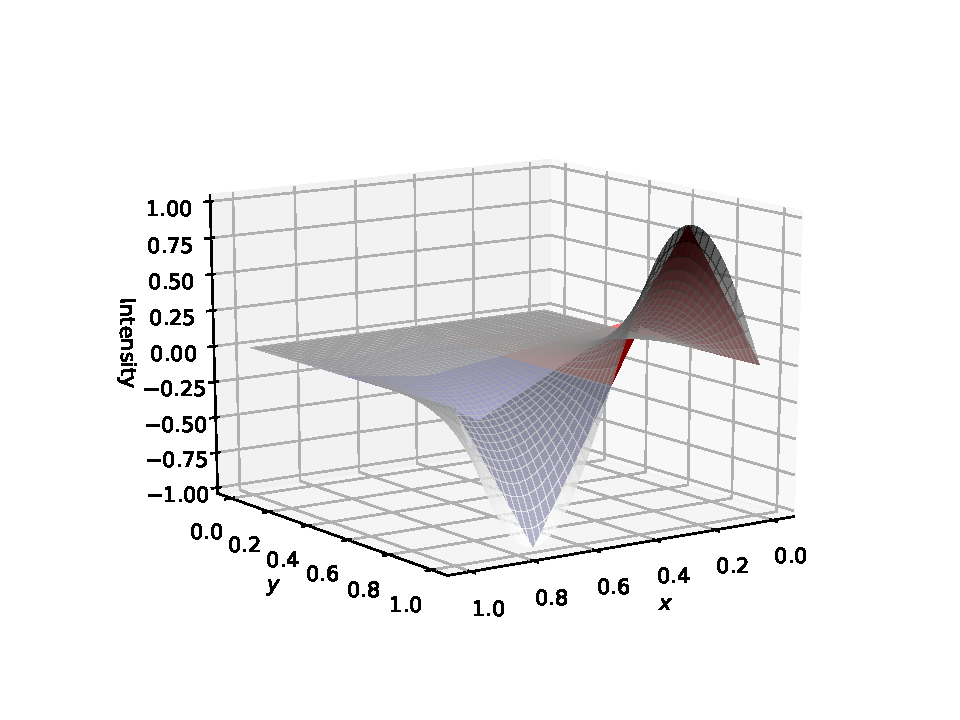
\includegraphics[width=0.9\linewidth]{plots/AnPlusNumSolM3Task3.pdf}\label{fig:task3M3}}\hspace{0mm}
\subfloat[$M_x = M_y = 50$]{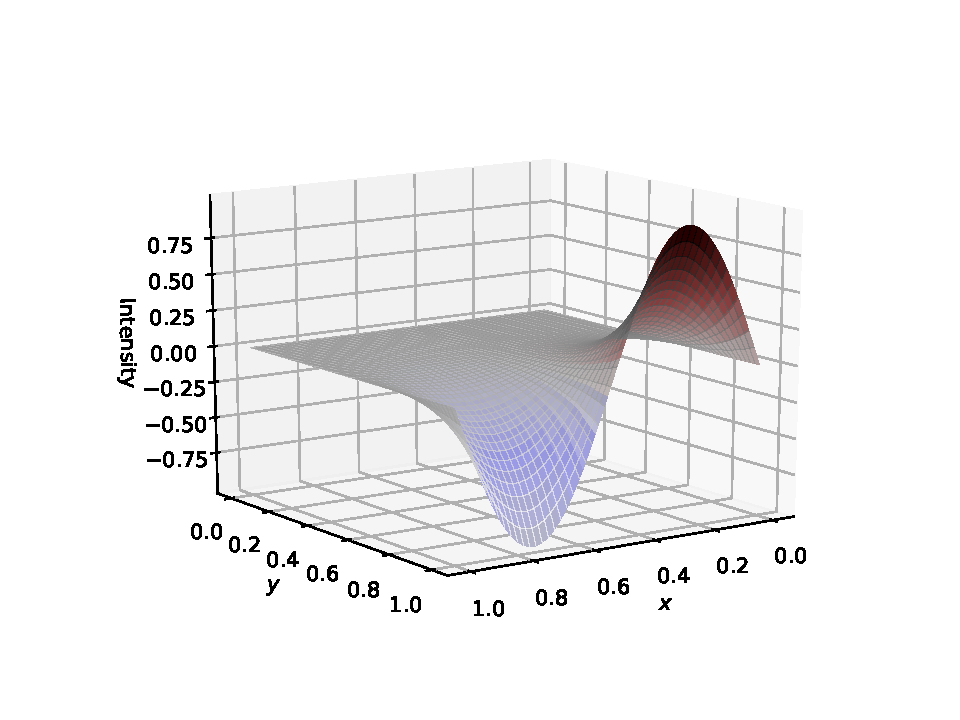
\includegraphics[width=0.9\linewidth]{plots/AnPlusNumSolM50Task3.pdf}\label{task3M50}}\hspace{0mm}
\caption{Two-Dimensional Laplace Equation, considered on the unit square. The analytical solution is shown in grey. The numerical solution is displayed in a \textit{seismic} color map. In (a), the numerical solution is calculated with $M_x = M_y = 3$, i.e. with 9 unknowns on a regular grid. In (b), the numerical solution is calculated with $M_x = M_y = 50$, i.e. with 2500 unknowns on a regular grid.}
\end{figure}
\newpage
In the next sections, the convergence of the numerical solution to the analytical solution will be quantified. Since the five point formula \eqref{fivePointFormula} uses a second order central difference approximation, as defined in section \ref{section_2.2}, in both directions $x$ and $y$, the truncation error is of order $\mathcal{O}(h^2 + k^2)$. The relative error $e^r_{\ell}$ for three different types of grids is displayed in "$\log$-$\log$"-convergence plots. The types of grids are 

\begin{itemize}
    \item $h$-refinement: $M_x$ increasing and $M_y$ constant
    \item $k$-refinement: $M_y$ increasing and $M_x$ constant
    \item $(h = k)$-refinement: Both $M_x$ and $M_y$ increasing at the same rate
\end{itemize}

\subsubsection*{Convergence with $h$-refinement}
Convergence plots for increasing $M_x$, with arbitrary constant values of $M_y$, are shown in figure \ref{subfigurestask3b1}. In all the cases presented, the convergence order is approximately $\mathcal{O}(N_{\mathrm{dof}}^{-2})$ up to a certain point, where the convergence order "flattens out". This matches the expected convergence rate, which is 

\begin{equation*}
\begin{split}
    \mathcal{O}(h^2 + k^2) &= \mathcal{O}(h^2) \overset{h \propto N_{\mathrm{dof}}^{-1}}= \mathcal{O}(N_{\mathrm{dof}}^{-2}), 
\end{split}
\end{equation*}
where $N_{\mathrm{dof}} = M_x\cdot M_y$. This is expected since $h$-refinement is being performed, which means that $k$ is assumed to be a small enough number such that $h$ will dominate the error. This is observed in practice when $M_x$ is increased. Note that the point where the convergence rate becomes asymptotic is shifted towards smaller errors and larger degrees of freedom when the constant $M_y$ is increased. This is clearly observed in the sequence of plots from (a) to (d). 

\begin{figure}[t]
\begin{subfigure}{.5\textwidth}
  \centering
  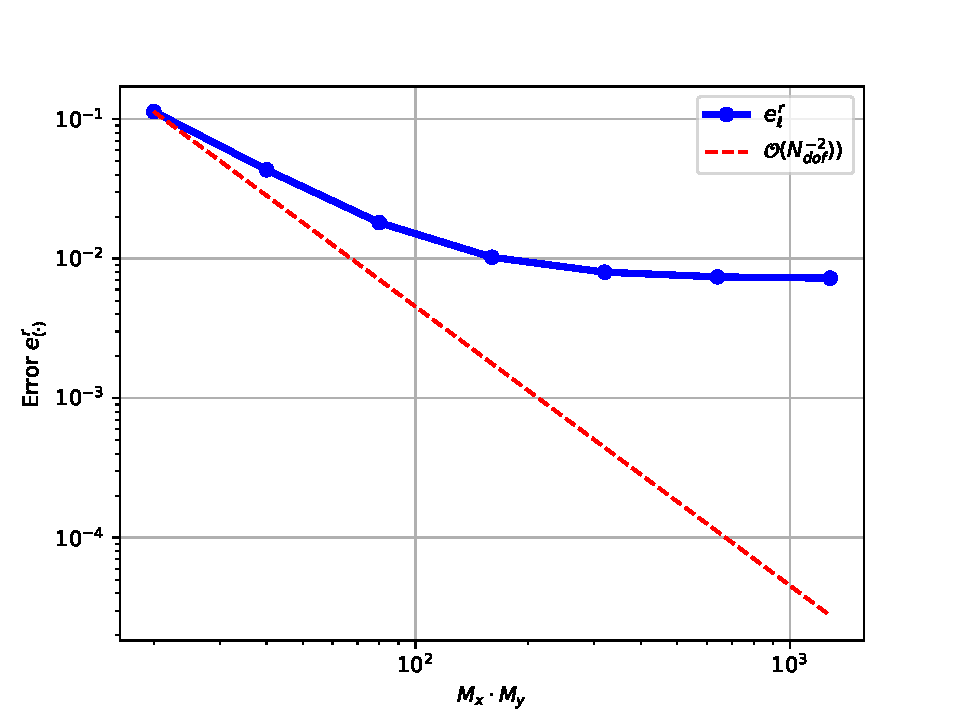
\includegraphics[width=\linewidth]{plots/task3bMy20.pdf}
  \caption{$M_y = 10$ and $M_x$ increasing}
\end{subfigure}
\begin{subfigure}{.5\textwidth}
  \centering
  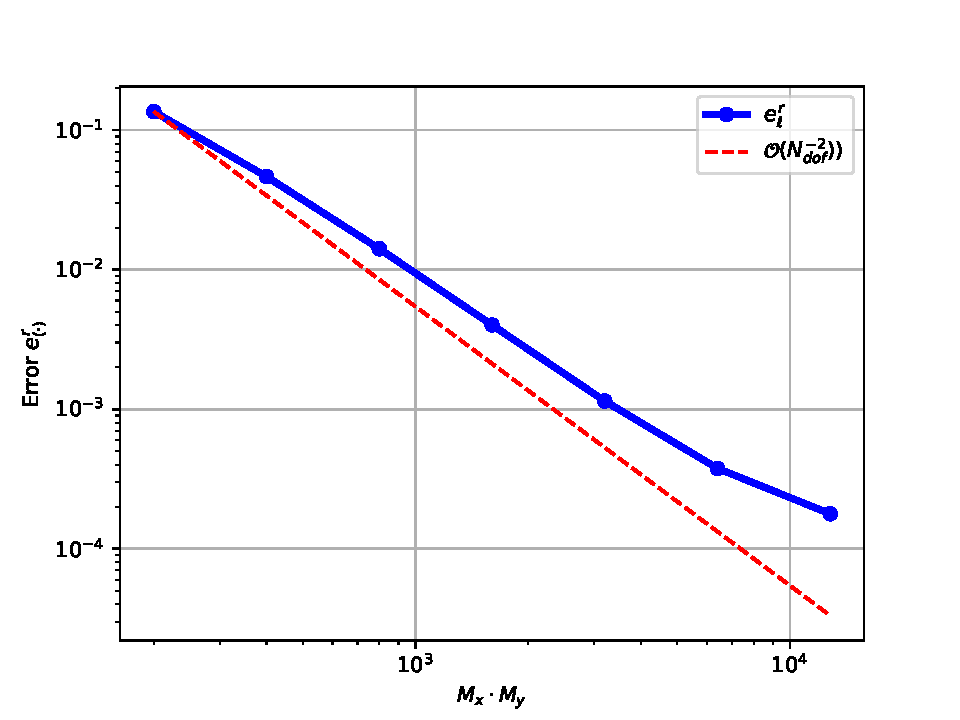
\includegraphics[width=\linewidth]{plots/task3bMy50.pdf}
  \caption{$M_y = 100$ and $M_x$ increasing}
\end{subfigure}
\begin{subfigure}{.5\textwidth}
  \centering
  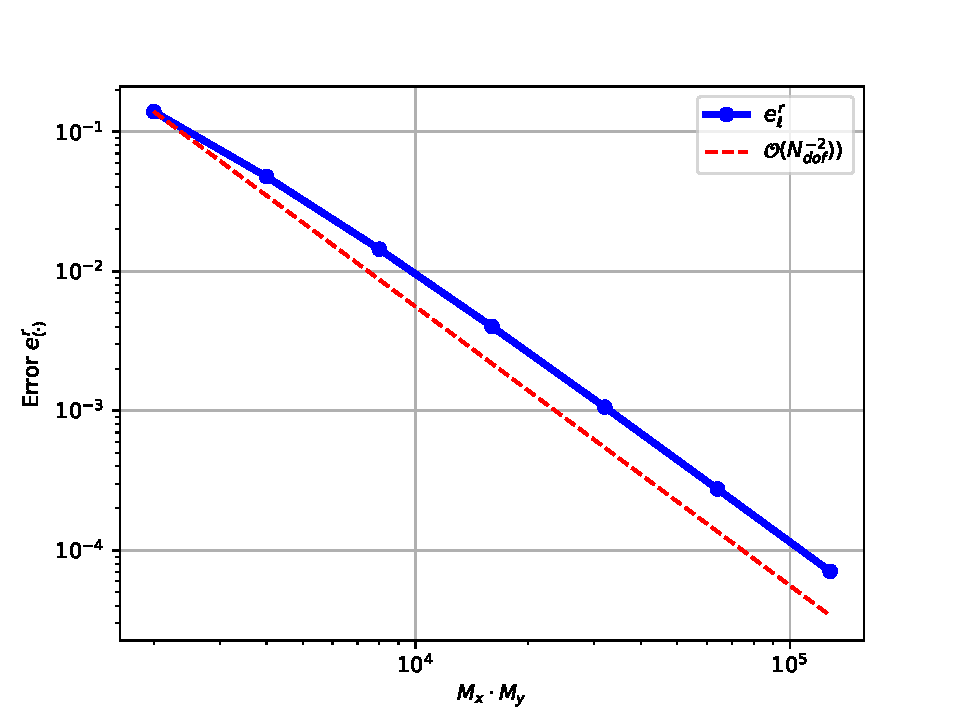
\includegraphics[width=\linewidth]{plots/task3bMy100.pdf}
  \caption{$M_y = 10^3$ and $M_x$ increasing}
\end{subfigure}
\begin{subfigure}{.5\textwidth}
  \centering
  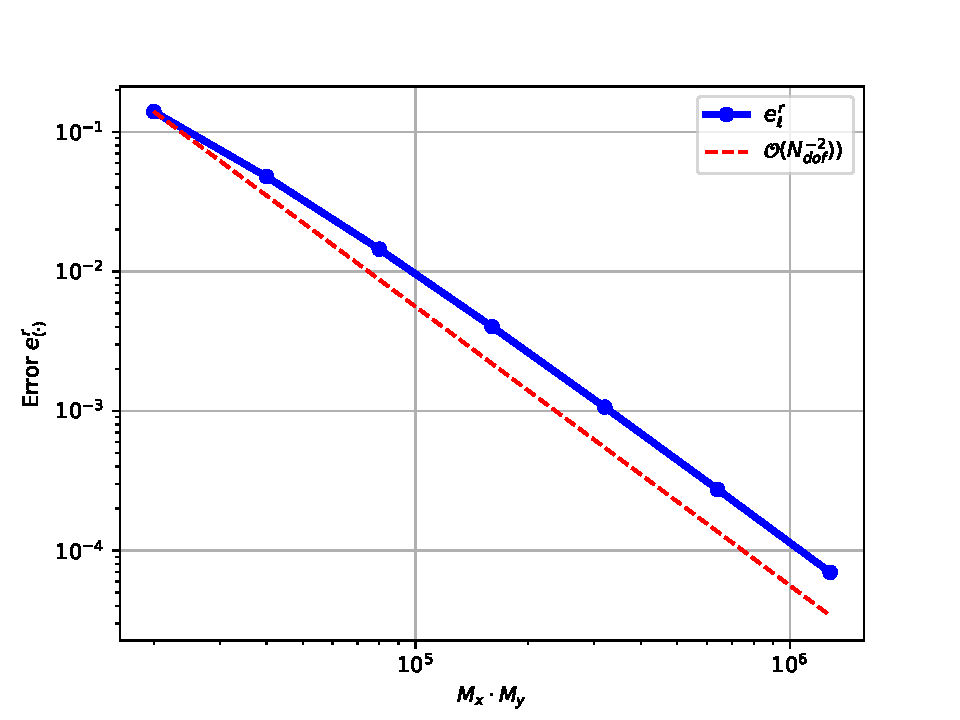
\includegraphics[width=\linewidth]{plots/task3bMy500.pdf}  \caption{$M_y = 10^4$ and $M_x$ increasing}
\end{subfigure}
\caption{Two-Dimensional Laplace Equation, considered on the unit square. The relative error $e^r_{\ell}$ is shown for some arbitrary constant values of $M_y$ and increasing $M_x$ ($h$-refinement). The $x$-axis shows $M_x \cdot M_y$, i.e. the number of degrees of freedom of the linear system.}
\label{subfigurestask3b1}
\end{figure}

\subsubsection*{Convergence with $k$-refinement}
Convergence plots for increasing $M_y$, with arbitrary constant values of $M_x$, are shown in figure \ref{subfigurestask3b2}. The expected convergence order, in this case, is

\begin{equation*}
\begin{split}
    \mathcal{O}(h^2 + k^2) &= \mathcal{O}(k^2) \overset{k \propto N_{\mathrm{dof}}^{-1}}= \mathcal{O}(N_{\mathrm{dof}}^{-2}). 
\end{split}
\end{equation*}
The reasoning of this expectation is similar as for $h$-refinement. In this case, $h$ is assumed to be a small number, such that the error stemming from $k$ will be asymptotically larger. In case (a) and (b), the expected convergence order of $\mathcal{O}(N_{\mathrm{dof}}^{-2})$ is not reached. The reason for this is that the constant $M_x$ is not large enough, which is assumed when neglecting the $h^2$-term when calculating the expected convergence order. Therefore, when the constant is increased, the expected convergence order is met, as observed in figures (c) and (d). Note that the point where the convergence rate becomes asymptotic is shifted towards larger errors and larger degrees of freedom when the constant $M_x$ is increased. Moreover, comparing to the plots in figure \ref{subfigurestask3b1}, it can be inferred that the refinement in the $x$-direction is crucial for reaching the expected convergence order. In other words, $x$ requires a finer grid compared to $y$. 

\begin{figure}[t]
\begin{subfigure}{.5\textwidth}
  \centering
  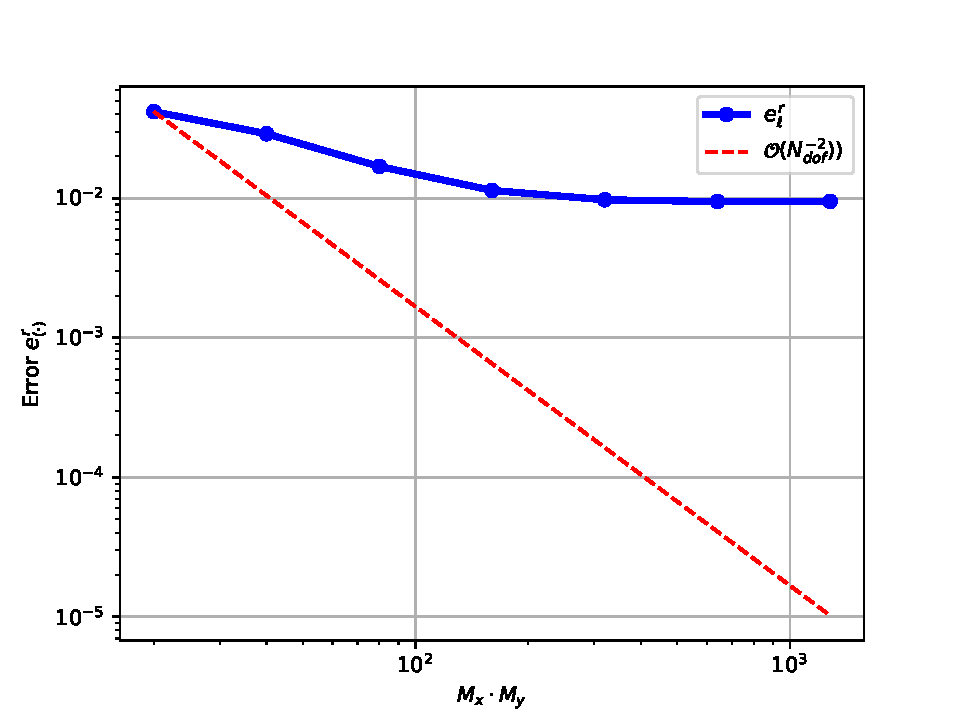
\includegraphics[width=\linewidth]{plots/task3bMx20.pdf}
  \caption{$M_x = 10$ and $M_y$ increasing}
\end{subfigure}
\begin{subfigure}{.5\textwidth}
  \centering
  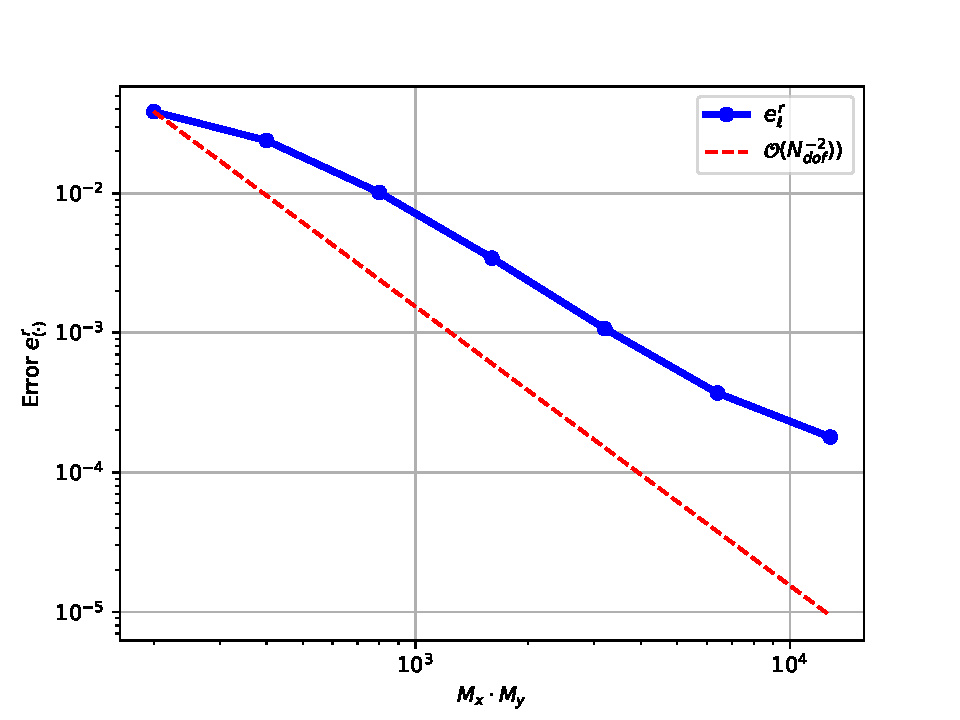
\includegraphics[width=\linewidth]{plots/task3bMx50.pdf}
  \caption{$M_x = 100$ and $M_y$ increasing}
\end{subfigure}
\begin{subfigure}{.5\textwidth}
  \centering
  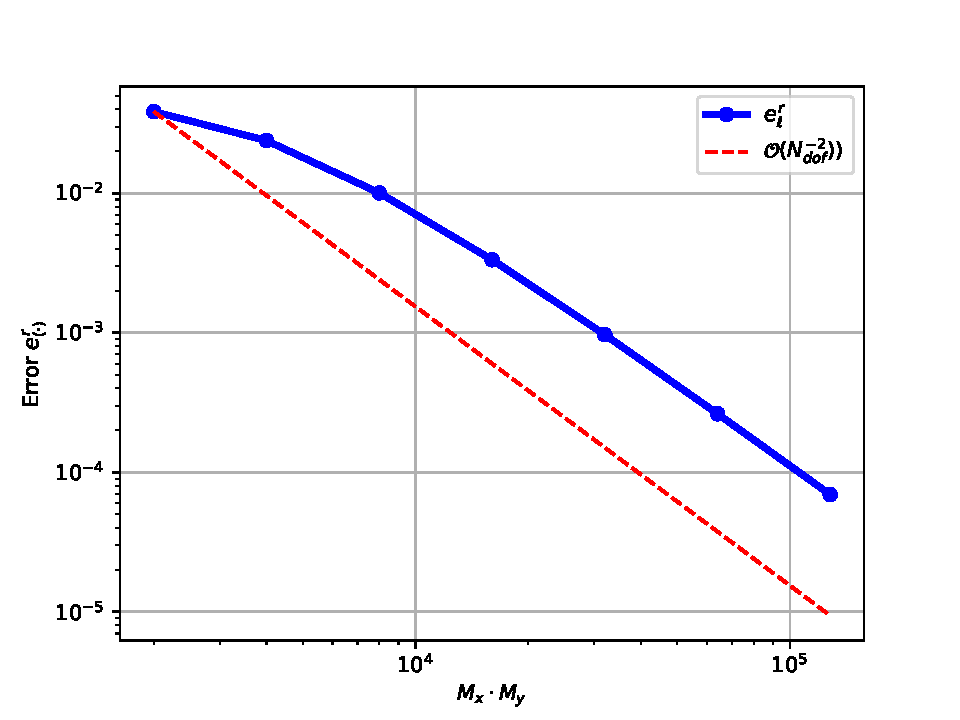
\includegraphics[width=\linewidth]{plots/task3bMx100.pdf}
  \caption{$M_x = 10^3$ and $M_y$ increasing}
\end{subfigure}
\begin{subfigure}{.5\textwidth}
  \centering
  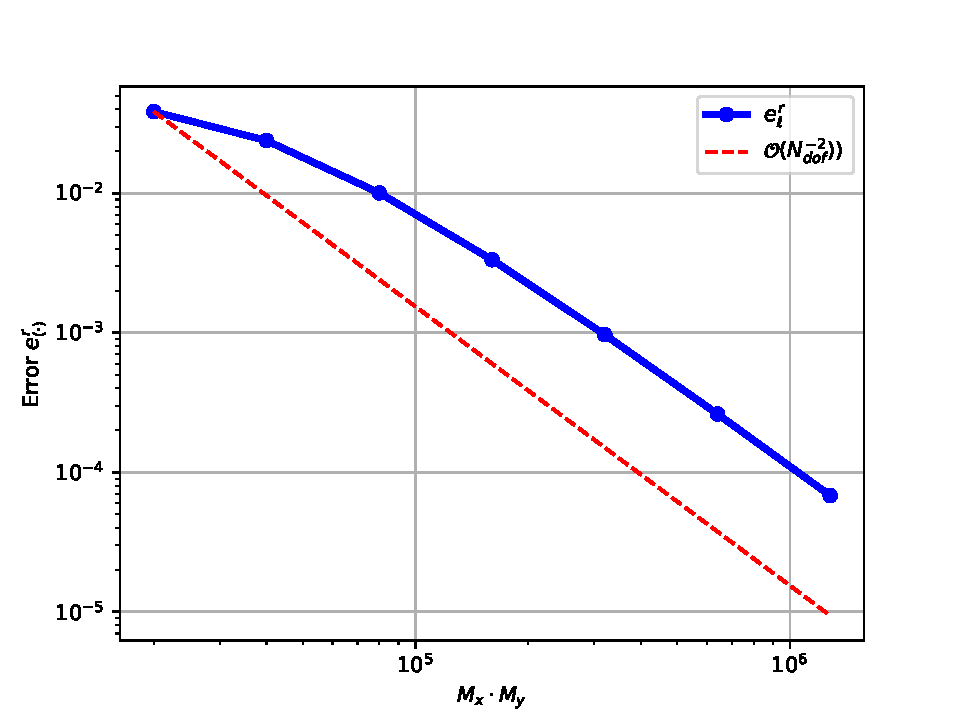
\includegraphics[width=\linewidth]{plots/task3bMx500.pdf}
  \caption{$M_x = 10^4$ and $M_y$ increasing}
\end{subfigure}
\caption{Two-Dimensional Laplace Equation, considered on the unit square. The relative error $e^r_{\ell}$ is shown for some arbitrary constant values of $M_x$ and increasing $M_y$ ($k$-refinement). The $x$-axis shows $M_x \cdot M_y$, i.e. the number of degrees of freedom of the linear system.}
\label{subfigurestask3b2}
\end{figure}

\subsubsection*{Convergence plot $(h = k)$-refinement}

A convergence plot where both $M_x$ and $M_y$ are increasing, at the same pace, i.e. $M_x = M_y$ at all times, is shown in figure \ref{task3bConvergenceBothVary}. As seen from the plot, the convergence order is approximately $\mathcal{O}(N_{\mathrm{dof}}^{-1})$. This is in accordance with the expected order of convergence, which is
\begin{equation*}
    \mathcal{O}(h^2+k^2) \overset{h = k} = \mathcal{O}(hk) = \mathcal{O}(N_{\mathrm{dof}}^{-1}).
\end{equation*}

\begin{figure}[t]
    \centering
    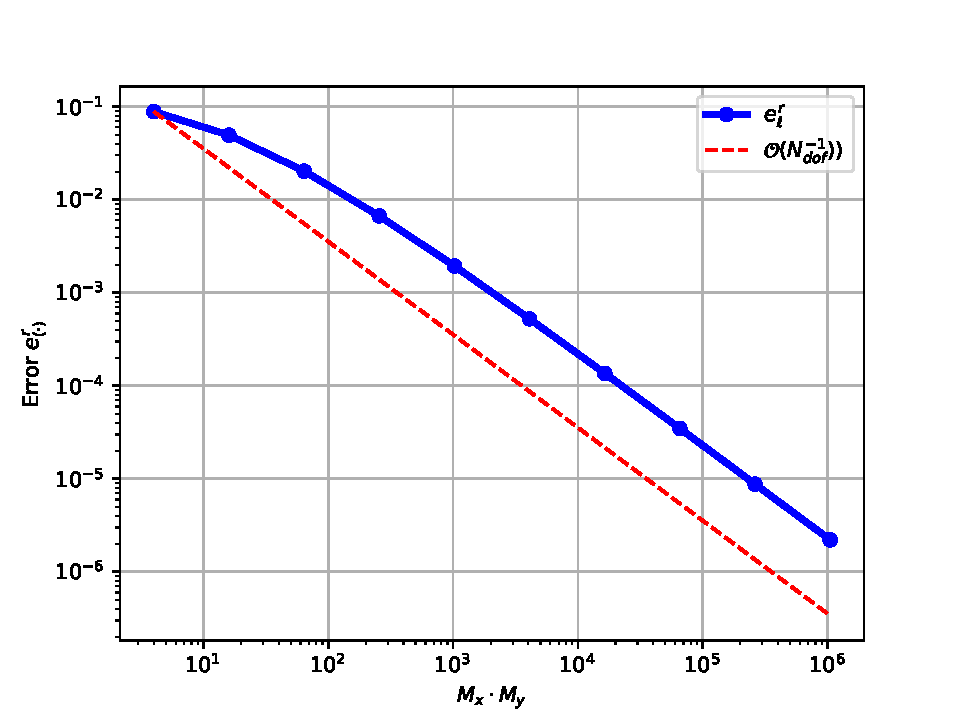
\includegraphics[width=0.85\linewidth]{plots/task3bBothVary.pdf}
    \caption{Two-Dimensional Laplace Equation, considered on the unit square. Plot of the relative error $e^r_{\ell}$ where both $M_x$ and $M_y$ are increasing monotonically ($(h=k)$-refinement). The $x$-axis shows $M_x \cdot M_y$, i.e. the number of degrees of freedom of the linear system.}
    \label{task3bConvergenceBothVary}
\end{figure}
\newpage
\ 
\newpage
\newpage
\ 
\newpage
